\documentclass[a4paper]{article}

% packages
\usepackage[utf8]{inputenc}
\usepackage[dutch]{babel}
\usepackage{hyperref}
\usepackage{graphicx}
\usepackage{glossaries}


% bibliografische databank
\usepackage[backend=biber, style=apa]{biblatex}
\DeclareLanguageMapping{dutch}{dutch-apa}
\addbibresource{stageverslag-2122.bib}


\makeglossaries
%%=============================================================================
%% Verklarende woordenlijst
%%=============================================================================
\newglossaryentry{kwartier}
{
    name=kwartier,
    description={Tijdelijke verblijfplaats voor militairen~\autocite{Wikipedia2021}},
    plural=kwartieren
}
\newglossaryentry{ccvc}
{
    name={CC V\&C},
    description={Competentie centrum Vliegend materieel \& Communicatie- en informatie-systemen}
}
\newglossaryentry{its}
{
    name=IT\&S,
    description={Information Technology \& Services}
}
\newglossaryentry{eenheid}
{
    name=eenheid,
    description={Een militaire eenheid bestaat uit een commando- en staf-element, uit uitvoerende militaire eenheden van een lager niveau en steuneenheden. Een militaire eenheid staat onder commando van een (onder)officier van voldoende rang~\autocite{Wikipedia2021a}},
    plural=eenheden
}
\newglossaryentry{lvm}
{
    name=LVM,
    description={Linux Volume Manager}
}
\newglossaryentry{rdp}
{
    name=RDP,
    description={Remote desktop protocol}
}
\newglossaryentry{acl}
{
    name=ACL,
    description={Access control list},
    plural={ACL's}
}
\newglossaryentry{selinux}
{
    name=SELinux,
    description={Security Enhanced Linux}
}
\newglossaryentry{db}
{
    name=db,
    description={Database},
    plural=db's
}

% Metadata
\title{Stageverslag}
\author{Pieter {Van Keer}}
\date{2021 - 2022}

\begin{document}
    
    % inhoudstafel
    \tableofcontents
    \pagebreak
    
    % kern
    %%=============================================================================
%% Voorwoord
%%=============================================================================
\section{Voorwoord}
\label{sec:voorwoord}

%% TODO:
%% Het voorwoord is het enige deel van de bachelorproef waar je vanuit je
%% eigen standpunt (``ik-vorm'') mag schrijven. Je kan hier bv. motiveren
%% waarom jij het onderwerp wil bespreken.
%% Vergeet ook niet te bedanken wie je geholpen/gesteund/... heeft



Dit stageverslag werd geschreven in het kader van de stage die ik liep bij Defensie van 21/02/2022 tot 27/05/2022. Dit was een zeer interessante periode omdat ik hier veel bijgeleerd heb.

Zoals vele andere dingen in het leven, kon ik dit niet alleen en daarom wil ik graag een aantal mensen bedanken. Steven beeckman, bedankt om mij zo goed te ontvangen bij Defensie, ook voor de vragen die ik had voor zowel de stage als bachelorproef kon ik steeds bij jou terecht. Tom De Leeuw, mijn stagementor, bedankt om mij te begeleiden en te helpen doorheen mijn stage. Wim De bruyn, mijn stagebegeleider, bedankt voor de opbouwende feedback en begeleiding tijdens de stage. Tot slot, Britt, die mij ondertussen al 3 jaar aanzet om het beste uit mezelf te halen.

\begin{flushleft}
    
Ik wens u veel leesplezier.
\end{flushleft}

\begin{flushleft}

Pieter Van Keer

Dendermonde, 27 mei, 2022

\end{flushleft}
    %%=============================================================================
%% Defensie
%%=============================================================================
%% stel stageplaats voor en schets waar je stage hebt gelopen.

\section{Defensie}
\label{sec:defensie}
%bron: https://www.mil.be/nl/over-defensie/#onze-organisatie
Defensie telt 26.179 personeelsleden, verdeeld over vier componenten: Landcomponent, Luchtcomponent, Marine en Medische Component. Daarnaast werken ze ook op de verschillende algemene directies en stafdepartementen, onder leiding van de Chef Defensie: admiraal Michel Hofman. Zie figuur~\ref{fig:organigram-defensie}

De personeelsleden van Defensie oefenen meer dan 300 verschillende beroepen uit. Dat maakt van Defensie een van de meest diverse werkgevers in het land, met zowel Nederlandstalige (54 \%) als Franstalige (46 \%) profielen. Militairen vormen de bulk van het personeelsbestand. Sommige functies vereisen echter geen uniform: bijna 6 \% ervan wordt ingevuld door burgerpersoneel. \autocite{Defensie2022}

\begin{figure}
    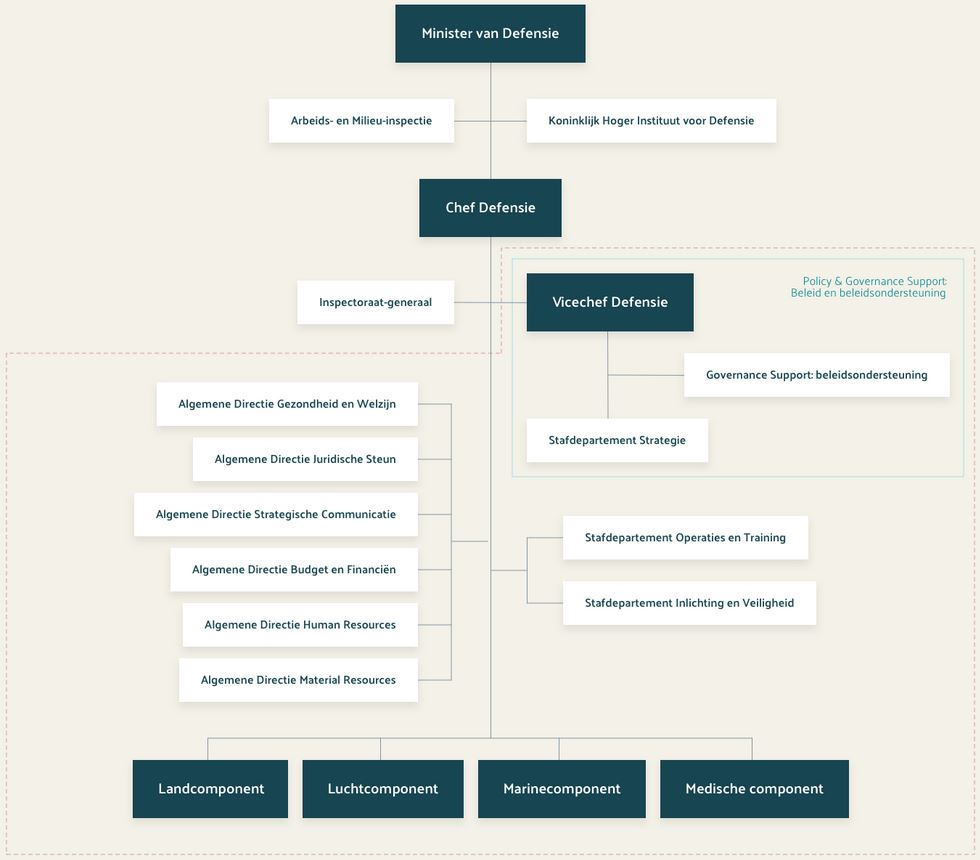
\includegraphics[width=\textwidth]{img/organigram-defensie.png}
    \caption{\label{fig:organigram-defensie}Organigram van Defensie~\autocite{Defensie2022}}
\end{figure}

\subsection{Stageplaats}

Defensie heeft verschillende \glspl{kwartier}, mijn stage vond plaats binnen de \gls{eenheid} \gls{ccvc} op het \gls{kwartier} Majoor Housiau gelegen te Peutie. Zie Figuur~\ref{fig:organigram-ccvc}

\begin{figure}
    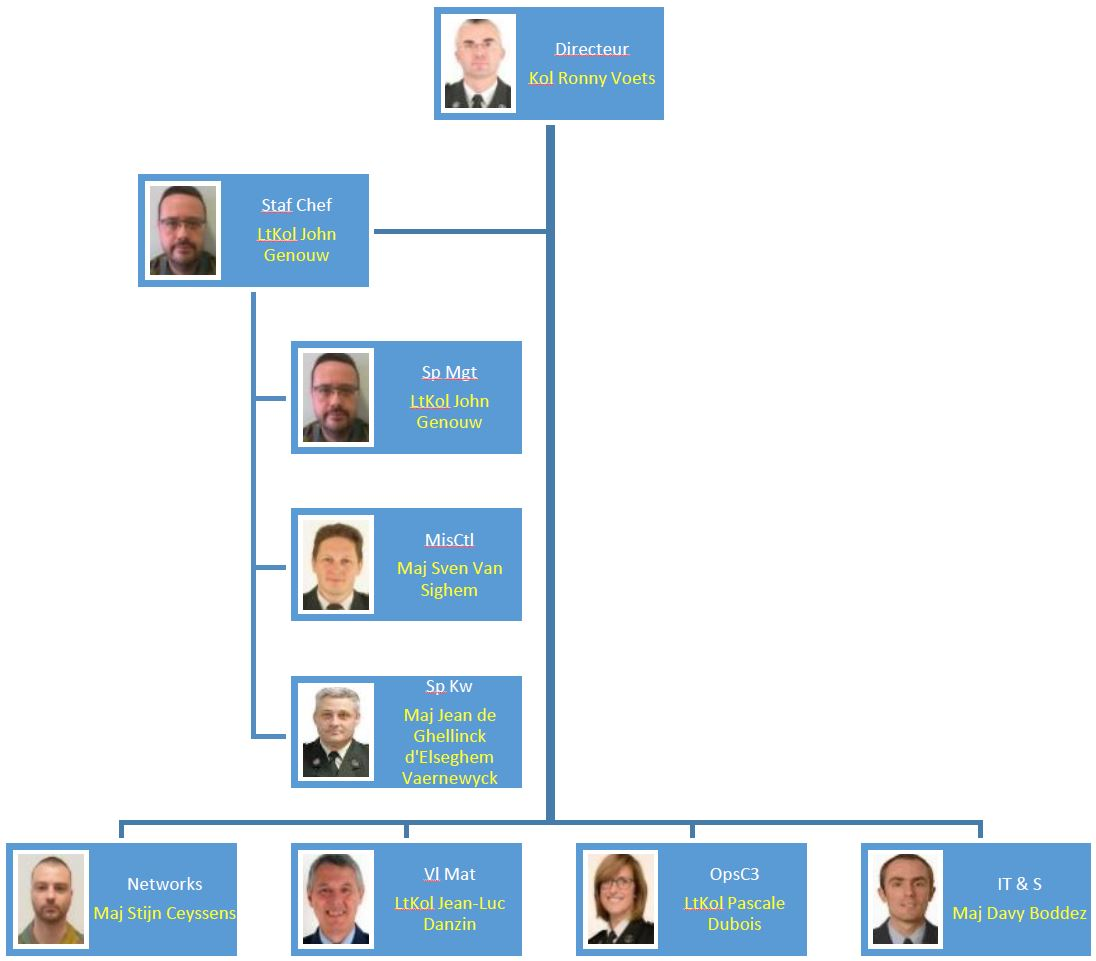
\includegraphics[width=\textwidth]{img/organigram-ccvc.png}
    \caption{\label{fig:organigram-ccvc}Organigram van de \gls{eenheid} \gls{ccvc}~\autocite{Defensie2022a}}
\end{figure}

Mijn stage was bij de afdeling Systems binnen het Departement \gls{its}. Zie figuur~\ref{fig:organigram-its}

\begin{figure}
    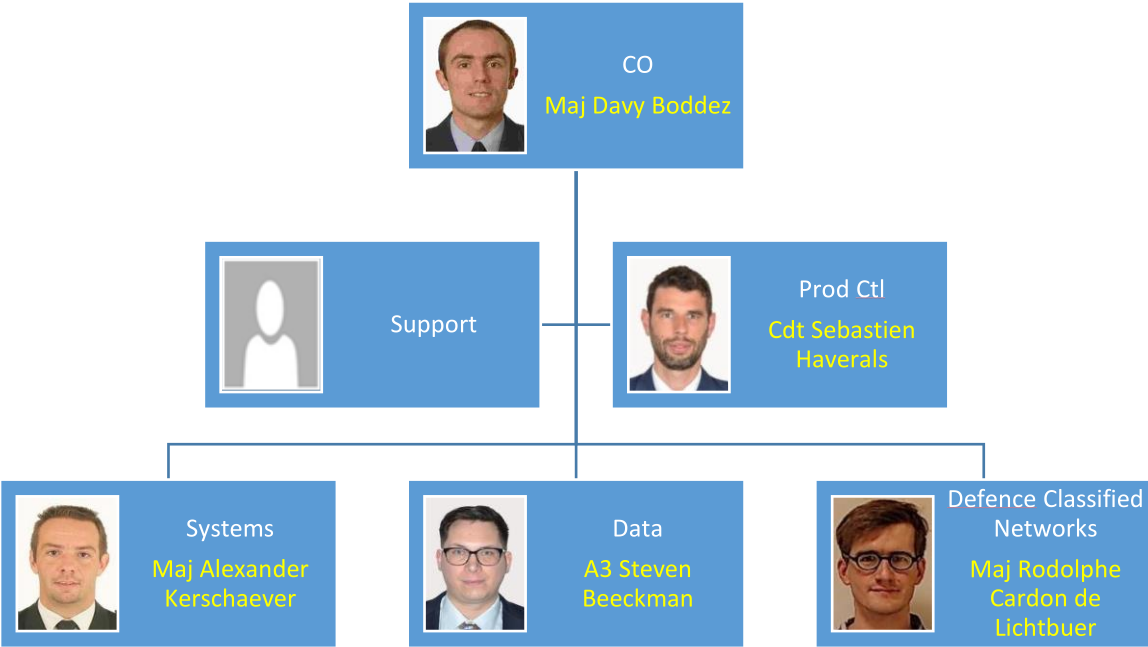
\includegraphics[width=\textwidth]{img/organigram-its.png}
    \caption{\label{fig:organigram-its}Organigram van het departement \gls{its}~\autocite{Defensie2022a}}
\end{figure}

Binnen de afdeling Systems zijn er 6 diensten:

\begin{itemize}
    \item linux
    \item windows
    \item oracle databanken
    \item Microsoft sql server
    \item prodctl
    \item techbu
\end{itemize}

Hoewel ik binnen elke dienst een introductie gekregen heb was miin stage vooral binnen de dienst linux.

Ik heb Defensie gekozen omdat ik ambitie heb om later bij Defensie te gaan werken. Op deze manier kan ik al eens kijken hoe het er aan toe gaat op de werkvloer.
    %%=============================================================================
%% Opdrachten
%%=============================================================================
% Opdracht template:

%\subsubsection{Beginsituatie}
%\subsubsection{Doel}
%\subsubsection{Plan van Aanpak}
%\subsubsection{Uitwerking}
%\subsubsection{Eindresultaat}
%\subsubsection{Business doelstellingen}
%\subsubsection{Persoonlijke doelstellingen}

\section{Opdrachten}
\label{sec:opdrachten}

\subsection{Backup-script moderniseren}

Binnen Defensie gebruikt men een bashscript genaamd ``bu\_script.sh'' om een backup te nemen van de databanken die bestaan op een machine en deze weg te schrijven op het netwerk.  
Ik kreeg de opdracht om dit script te moderniseren. Om de opdracht een beetje te vereenvoudigen moest ik de backup's lokaal wegschrijven.

\subsubsection{Beginsituatie}

Het script bestaat maar het is verouderd. Met het script is het mogelijk om meerdere instances van Mariadb/mysql te backuppen. Het script is zeer lang en moeilijk leesbaar.

\subsubsection{Doel}

\begin{itemize}
    \item moderniseer het script
    \item maak het script meer flexibel door gebruik te maken van meer variabelen
    \item genereer een rapport van de uitvoering van het script
    \item schrijf de backup lokaal weg onder de map ``$\sim$/backup''
\end{itemize}

\subsubsection{Plan van Aanpak}

\begin{enumerate}
    \item lees het script door en probeer de denkwijze te begrijpen van de persoon die het script geschreven heeft
    \item verwijder delen die niet meer van toepassing zijn
    \item voeg meer commentaar toe aan het script zodat iemand die het script later zal doornemen sneller weet wat er gebeurd
    \item gebruik meer functies aan zodat het script meer leesbaar wordt
    \item test het script
\end{enumerate}

\subsubsection{Uitwerking}

Ik ben begonnen met het script door te nemen en de logica proberen te verstaan. Tijdens dat ik dit deed heb ik extra commentaar geschreven om duidelijk te maken wat er juist gebeurde in het script. Na een kort gesprek met Tom hebben we besloten om het script enkel te beperken voor server die maar 1 instance hebben van mariadb/mysql. Hierdoor werd het script al veel meer leesbaar. Door extra hulpfuncties toe te voegen is de leesbaarheid ook verbeterd. Tijdens het testen heb ik er nog enkele bugs uitgehaald maar het script werkt zoals gevraagd.

\subsubsection{Eindresultaat}

Het eindresultaat is een script dat makkelijker te lezen/verstaan en flexibel is. Het script gaat een rapport genereren van de uitvoering en de backup was te vinden in de map ``$\sim$/backup''. Er is mogelijkheid om in te toekomst het script uit te breiden zodat dit een melding gaat genereren in Zabbix (monitoring tool).

\subsubsection{Business doelstellingen}

Voor de business was het belangrijk dat het script een moderne update kreeg. Dit was zeker het geval.

\subsubsection{Persoonlijke doelstellingen}

Voor mij persoonlijk was dit een geslaagde opdracht. Het script is nu meer flexibel en dit zal er voor zorgen dat men dit in de toekomst nog kan uitbreiden.


\subsection{Procedure upgrade mariadb}

Tegen 2024 moeten alle dbserver binnen Defensie draaien op Mariadb 10.6 op RHEL 8. Om deze transitie rustig te laten verlopen is er nood aan een procedure die men kan volgen tijdens zo een upgrade van een machine.

\subsubsection{Beginsituatie}

De dbserver bij Defensie draaien op mariadb 5.5 op RHEL 7.

\subsubsection{Doel}

Schrijf een procedure die men kan volgen om een machine te upgraden naar Mariadb 10.6 op RHEL 8. De procedure moet aandacht schenken aan volgende punten:

\begin{itemize}
    \item het besturingssysteem van de nieuwe machine is Red Hat Enterprise Linux (RHEL) 8
    \item er gaat geen data verloren
    \item de juiste mensen inlichten dat er onderhoud zal doorgevoerd worden op hun dbserver
\end{itemize}

\subsubsection{Plan van Aanpak}

Voor deze opdracht zal ik iteratief werken:

\begin{itemize}
    \item de eerste iteratie zal ik op papier (in grote lijnen) schetsen wat er moet gebeuren
    \item de tweede iteratie zal ik dit in een word-document gieten en laten nalezen door Tom
    \item de derde en volgende iteratie(s) zal ik de procedure meer specifiek maken
\end{itemize}

\subsubsection{Uitwerking}
\subsubsection{Eindresultaat}
\subsubsection{Business doelstellingen}
\subsubsection{Persoonlijke doelstellingen}

\subsection{High availability bij databanken}


Onderzoek hoe men binnen defensie high availability implementeren? Als er een db faalt en niet beschikbaar is moet de applicatie zonder problemen verderwerken. Volgende punten moeten zeker vermeld zijn:

\begin{itemize}
    \item is er een licentie voor nodig?
    \item is de software ondersteund door Red Hat?
    \item zijn er open source beperkingen?
    \begin{itemize}
        \item enkel voor commercieel gebruik?
        \item beperking voor militaire doeleinden?
    \end{itemize}
\end{itemize}

\subsubsection{Beginsituatie}

Binnen Defensie is er momenteel maar 1 databank achter een bepaalde applicatie. Dit zorgt er natuurlijk voor dat als die databank faalt, de applicatie ook niet meer zal werken.

\subsubsection{Doel}

Zorg ervoor dat er meerdere databanken met dezelfde data achter een bepaalde applicatie zitten.

\subsubsection{Plan van Aanpak}

Voor deze opdracht zal ik iteratief werken:

\begin{itemize}
    \item de eerste iteratie zal ik op papier (in grote lijnen) schetsen wat er moet gebeuren alsook ideeën opschrijven van productie die men mogelijk kan gebruiken
    \item de tweede iteratie zal ik dit in een word-document gieten en laten nalezen door Tom
    \item de derde en volgende iteratie(s) zal ik de procedure meer specifiek maken en uitbreiden
\end{itemize}

Nadat het document volledig is ga ik een handleiding maken om dit te implementeren en een eenvoudige opstelling testen met 2 servers.

\subsubsection{Uitwerking}
\subsubsection{Eindresultaat}
\subsubsection{Business doelstellingen}
\subsubsection{Persoonlijke doelstellingen}

\subsection{MS SQL logins}

\subsubsection{Beginsituatie}

De Jboss Application servers connecteren zich met MSSQL server met SQL logins en dus via SQL server authentication.

\subsubsection{Doel}

Voer een onderzoek en beantwoord volgende vragen:

\begin{itemize}
    \item Kan Windows authentication gebruikt worden?
    \item Wat zijn mogelijke alternatieven voor Authenticatie?
    \begin{itemize}
        \item Wat zijn voor- en nadelen (vooral op vlak van Security en Management)?
    \end{itemize}
    \item Welke configuratie/software/drivers moet er geïnstalleerd worden om dit mogelijk te maken?
\end{itemize}

\subsubsection{Plan van Aanpak}

Ik ga beginnen met mezelf bekend te maken met het onderwerp. Ik ga een virtuele machine vragen waar ik op kan testen. Daarna zal ik een oplossing proberen zoeken op het probleem, en als laatste zal ik deze testen.

%\subsubsection{Uitwerking}
%\subsubsection{Eindresultaat}
\subsubsection{Business doelstellingen}

Door het gebruikt van windows authentication zal het systeem veiliger worden.

%\subsubsection{Persoonlijke doelstellingen}
    %%=============================================================================
%% Eindereflectie
%%=============================================================================
\section{Eindreflectie}
\label{sec:Eindreflectie}

\subsection{Voldoet de stage aan hetgeen ik verwacht had?}

Ja, ik ben terecht gekomen bij toffe mensen die me met open armen ontvangen hebben. Het was een unieke ervaring om te werken in een militaire sfeer.

\subsection{Overwelke opdracht ben ik het meest trots?}

De procedure om mariadb te upgraden, daar ben ik het meest trots op. Ik heb een script geschreven in Python terwijl ik redelijk weinig ervaring heb met Python. Ook heb ik hier veel bijgeleerd, qls je ook een upgrade van een besturingssysteem moet doen dan is de upgrade minder vanzelfsprekend 

\subsection{Is dit het toekomstbeeld dat ik voor ogen heb?}

Ja, werken met linuxservers zie ik me in de toekomst zeker nog doen maar ik denk dat er ook andere dingen zijn die ik eens wil proberen zoals bijvoorbeeld \gls{ci}/\gls{cd} voorzien in een DevOps project.

\subsection{Vind je van jezelf dat je genoeg ervaring hebt opgedaan om nu in het werkveld te stappen?}

Zeker en vast, Ik heb veel bijgeleerd over linuxservers en het beheer ervan. Ook de provisioning van de server begrijp ik nu beter. Uiteraard als je bij een andere werkgever toekomst zal je sowieso even moeten aanpassen aan de manier van werken vooraleer je het beste uit jezelf kan halen.
    \pagebreak
    
    %Referentielijst
    \printbibliography
    \pagebreak
    
    % Verklarende woordenlijst
    \printglossary[title=Verklarende woordenlijst, toctitle=Verklarende woordenlijst]
    \pagebreak
    
    \appendix
    %
\hypertarget{stage-logboek-week-1-21022022---24022022}{%
\section{Stage logboek: Week 1 (21/02/2022 -
24/02/2022)}\label{stage-logboek-week-1-21022022---24022022}}

\hypertarget{maandag-21022022}{%
\subsection{Maandag 21/02/2022}\label{maandag-21022022}}

\emph{Eerste stagedag}. Kennismaking met \textbf{Tom De Leeuw}, Tom
staat in voor het linuxgedeelte. Laptop ontvangen, vooral gepraat over
mogelijkheden van de stage.

Werkwijze voor telewerken:

\begin{enumerate}
\def\labelenumi{\arabic{enumi}.}
\tightlist
\item
  surf naar \url{https://portal.connect.mil.be} en meld aan met
  \textbf{itsme}
\item
  Kies voor vpn. Eens de verbinding opstaat kan je beginnen met skype.
\end{enumerate}

\hypertarget{dinsdag-22022022}{%
\subsection{Dinsdag 22/02/2022}\label{dinsdag-22022022}}

werkuren: \emph{8:00 - 16:00}

Zelfstandig research gedaan naar LVM (Linux Volume manager)
--\textgreater{}
\url{https://access.redhat.com/documentation/en-us/red_hat_enterprise_linux/8/html/configuring_and_managing_logical_volumes/index}
Na de research enkele kleine opdrachtjes uitgevoerd op mijn eigen
devserver binnen Defensie:

\begin{enumerate}
\def\labelenumi{\arabic{enumi}.}
\tightlist
\item
  Aanmaken logical volume

  \begin{itemize}
  \tightlist
  \item
    Maak logical volume aan van 300mb
  \item
    mount logical volume op \texttt{/var/data01}
  \item
    herstart server en kijk of het nog bestaat.
  \end{itemize}
\item
  Aanpassen logical volume

  \begin{itemize}
  \tightlist
  \item
    vergroot logical volume
  \item
    verklein logical volume
  \end{itemize}
\item
  Volume groups

  \begin{itemize}
  \tightlist
  \item
    maak 2 volume groups van 100-200mb
  \end{itemize}
\end{enumerate}

Achteraf als afsluiter van de dag moest ik een grafische omgeving
installeren op mijn devserver en proberen om via windows rdp de server
te kunnen overnemen.

\hypertarget{woensdag-23022022}{%
\subsection{Woensdag 23/02/2022}\label{woensdag-23022022}}

werkuren: \emph{8:00 - 16:00}

Zelfstandig research gedaan naar
\href{https://www.redhat.com/en/technologies/management/satellite}{Redhat
Satellite}, \href{https://theforeman.org}{Foreman} en
\href{https://www.theforeman.org/plugins/katello/}{Katello}. Ook naar
filesecurity: ACL's, SELinux

Verworven kennis toegepast in demo-omgeving. Samen met Tom de Satellite
omgeving ontdekt. uitleg gekregen hoe alles werkt.

\hypertarget{donderdag-24022022}{%
\subsection{Donderdag 24/02/2022}\label{donderdag-24022022}}

werkuren: \emph{8:00 - 16:00}

Kennis opgefrist ivm Mariadb, mysql en appstreams in RHEL. Manueel
mariadb geïnstalleerd op devmachine, db en users aangemaakt. Research
over puppet en aan de hand van puppet mariadb proberen installeren en
users en db's aan te maken. Meeting bijgewoond met externe mensen.


    %
\hypertarget{stage-logboek-week-2-28022022---04032022}{%
\section{Stage logboek: Week 2 (28/02/2022 -
04/03/2022)}\label{stage-logboek-week-2-28022022---04032022}}

\hypertarget{maandag-28022022}{%
\subsection{Maandag 28/02/2022}\label{maandag-28022022}}

werkuren: \emph{08:00-16:00}

Afgewerkt waar ik vorige donderdag mee bezig was. Bezig aan het
moderniseren van het script \texttt{bu\_script.sh}.

\hypertarget{dinsdag-01032022}{%
\subsection{Dinsdag 01/03/2022}\label{dinsdag-01032022}}

werkuren: \emph{8:00 - 16:00}

\texttt{bu\_script.sh} afgewerkt. Eenvoudige zelfgeschreven versie.\\
Begin aan voorbereiding theorie voor donderdag.

\hypertarget{woensdag-02032022}{%
\subsection{Woensdag 02/03/2022}\label{woensdag-02032022}}

werkuren: \emph{8:00 - 16:00}

Voorbereiding voor Donderdag

\begin{itemize}
\tightlist
\item
  Research gedaan in verband met
  \href{https://www.zabbix.com/documentation/5.0/en/manual/introduction/about}{Zabbix}
  (monitoring tool)
\item
  Git kennis opgefrist
\item
  Toegang gekregen tot de gitlab servers van Defensie.
\item
  Hello world project geschreven in Puppet op mijn dev machine
\end{itemize}

\hypertarget{donderdag-03032022}{%
\subsection{Donderdag 03/03/2022}\label{donderdag-03032022}}

werkuren: \emph{8:00 - 16:00}

Introductie tot Zabbix en puppet door Donovan. Daarna zelf via puppet
zabbix proberen installeren op devmachine.


    %
\hypertarget{stage-logboek-week-3-07032022---11032022}{%
\section{Stage logboek: Week 3 (07/03/2022 -
11/03/2022)}\label{stage-logboek-week-3-07032022---11032022}}

\hypertarget{maandag-07032022}{%
\subsection{Maandag 07/03/2022}\label{maandag-07032022}}

werkuren: \emph{08:00-16:00}

\begin{itemize}
\tightlist
\item
  Denk oefening:

  \begin{itemize}
  \tightlist
  \item
    Hoe kan je het \texttt{bu\_script.sh} uitbreiden zodat er een
    melding komt in Zabbix wanneer een backup faalt?
  \item
    Zoek uit wat er misgegaan is met de devmachine (te weinig geheugen)
  \end{itemize}
\end{itemize}

\hypertarget{dinsdag-08032022}{%
\subsection{Dinsdag 08/03/2022}\label{dinsdag-08032022}}

werkuren: \emph{8:00 - 16:00}

Introductie in Jboss applicatie servers door Christophe. Christophe
heeft me alles goed uitgelegd en we hebben een testapplicatie gedeployed
op mijn devmachine. Ik heb (onder begeleiding van Christophe) een
applicatie mogen vernieuwen in de acceptatieomgeving. (netmanto)

\hypertarget{woensdag-09032022}{%
\subsection{Woensdag 09/03/2022}\label{woensdag-09032022}}

werkuren: \emph{8:00 - 16:00}

De introductie in Jboss Applicatie servers verder gezet en afgewerkt. We
hebben nu niet alles maar redelijk veel overlopen van jboss servers. Ook
is het nu duidelijk hoe deze gemonitord worden (Jboss Operations
Networks).

Een eerste stagegesprek.

\hypertarget{donderdag-10032022}{%
\subsection{Donderdag 10/03/2022}\label{donderdag-10032022}}

Werkuren: \emph{08:30 - 16:30}

Werkdag in Peutie.

De opdracht gekregen om een oplossing te zoeken voor volgende problemen:

\begin{itemize}
\tightlist
\item
  Hoe high availability implementeren voor een db die aan een applicatie
  hangt?
\item
  Maak een procedure om Mariadb 5.5 op RHEL 7.x to upgraden naar Mariadb
  10.6 op RHEL 8 zonder verlies van gegevens.
\end{itemize}

Ook de toegangsbadge in orde gemaakt samen met Donovan.


    %
\hypertarget{stage-logboek-week-4-14032022---18032022}{%
\section{Stage logboek: Week 4 (14/03/2022 -
18/03/2022)}\label{stage-logboek-week-4-14032022---18032022}}

\hypertarget{maandag-14032022}{%
\subsection{Maandag 14/03/2022}\label{maandag-14032022}}

werkuren: \emph{08:00-16:00}

Verder gewerkt aan de denkoefeningen op een iteratieve manier. Alles
mooi in een word-documentje gegoten.

\hypertarget{dinsdag-15032022}{%
\subsection{Dinsdag 15/03/2022}\label{dinsdag-15032022}}

werkuren: \emph{8:00 - 16:00}

Verder gewerkt aan de denkoefeningen op een iteratieve manier. Er is
nood aan validatie van gebruikers en databanken. Hiervoor een concept
bedacht.

\hypertarget{woensdag-16032022}{%
\subsection{Woensdag 16/03/2022}\label{woensdag-16032022}}

werkuren: \emph{8:00 - 16:00}

Verder gewerkt aan de denkoefeningen.

Upgrade mariadb:

\begin{itemize}
\tightlist
\item
  Validatie voor users bedacht. gestart aan een script om dit uit te
  voeren maar ik zat vast gaandeweg dus nu ga ik eens kijken dat er geen
  andere manier is om dit te doen.
\end{itemize}

db high availability:

\begin{itemize}
\tightlist
\item
  Iteratie afgewerkt. Nu wachten op feedback.
\end{itemize}

Stageverslag: structuur opgemaakt.

\hypertarget{donderdag-17032022}{%
\subsection{Donderdag 17/03/2022}\label{donderdag-17032022}}

Werkuren: \emph{08:15 - 16:15}

Fysiek in Peutie.

Normaal was er een introductie van mssql gepland vandaag maar deze is
verzet naar een later moment. Ter vervanging heb ik verschillende
praktische oefeningen gedaan ivm LVM op mijn devmachine. Ook dit
allemaal besproken met Tom.


    %% Options for packages loaded elsewhere
\PassOptionsToPackage{unicode}{hyperref}
\PassOptionsToPackage{hyphens}{url}
%
\documentclass[
]{article}
\usepackage{amsmath,amssymb}
\usepackage{lmodern}
\usepackage{iftex}
\ifPDFTeX
  \usepackage[T1]{fontenc}
  \usepackage[utf8]{inputenc}
  \usepackage{textcomp} % provide euro and other symbols
\else % if luatex or xetex
  \usepackage{unicode-math}
  \defaultfontfeatures{Scale=MatchLowercase}
  \defaultfontfeatures[\rmfamily]{Ligatures=TeX,Scale=1}
\fi
% Use upquote if available, for straight quotes in verbatim environments
\IfFileExists{upquote.sty}{\usepackage{upquote}}{}
\IfFileExists{microtype.sty}{% use microtype if available
  \usepackage[]{microtype}
  \UseMicrotypeSet[protrusion]{basicmath} % disable protrusion for tt fonts
}{}
\makeatletter
\@ifundefined{KOMAClassName}{% if non-KOMA class
  \IfFileExists{parskip.sty}{%
    \usepackage{parskip}
  }{% else
    \setlength{\parindent}{0pt}
    \setlength{\parskip}{6pt plus 2pt minus 1pt}}
}{% if KOMA class
  \KOMAoptions{parskip=half}}
\makeatother
\usepackage{xcolor}
\IfFileExists{xurl.sty}{\usepackage{xurl}}{} % add URL line breaks if available
\IfFileExists{bookmark.sty}{\usepackage{bookmark}}{\usepackage{hyperref}}
\hypersetup{
  hidelinks,
  pdfcreator={LaTeX via pandoc}}
\urlstyle{same} % disable monospaced font for URLs
\usepackage{graphicx}
\makeatletter
\def\maxwidth{\ifdim\Gin@nat@width>\linewidth\linewidth\else\Gin@nat@width\fi}
\def\maxheight{\ifdim\Gin@nat@height>\textheight\textheight\else\Gin@nat@height\fi}
\makeatother
% Scale images if necessary, so that they will not overflow the page
% margins by default, and it is still possible to overwrite the defaults
% using explicit options in \includegraphics[width, height, ...]{}
\setkeys{Gin}{width=\maxwidth,height=\maxheight,keepaspectratio}
% Set default figure placement to htbp
\makeatletter
\def\fps@figure{htbp}
\makeatother
\setlength{\emergencystretch}{3em} % prevent overfull lines
\providecommand{\tightlist}{%
  \setlength{\itemsep}{0pt}\setlength{\parskip}{0pt}}
\setcounter{secnumdepth}{-\maxdimen} % remove section numbering
\ifLuaTeX
  \usepackage{selnolig}  % disable illegal ligatures
\fi

\author{}
\date{}

\begin{document}

\hypertarget{stage-logboek-week-5-21032022---25032022}{%
\section{Stage logboek: Week 5 (21/03/2022 -
25/03/2022)}\label{stage-logboek-week-5-21032022---25032022}}

\hypertarget{maandag-21032022}{%
\subsection{Maandag 21/03/2022}\label{maandag-21032022}}

werkuren: \emph{08:00-16:00}

Verder gewerkt aan de denkoefening om high availability te implementeren
bij databanken. Tom heeft voor mij een aantal virtuele machines laten
maken zodat ik hierop kan testen.

Stageverslag verder aangevuld.

\hypertarget{dinsdag-22032022}{%
\subsection{Dinsdag 22/03/2022}\label{dinsdag-22032022}}

Geen stage.\\
Jobevent van HoGent

\hypertarget{woensdag-23032022}{%
\subsection{Woensdag 23/03/2022}\label{woensdag-23032022}}

werkuren: \emph{8:00 - 16:00}

Verder gewerkt aan de denkoefening om high availability te implementeren
bij databanken: Testopstelling gemaakt.

\begin{itemize}
\tightlist
\item
  databank master
\item
  databank slave
\item
  reverse proxy
\end{itemize}

\begin{figure}
\centering
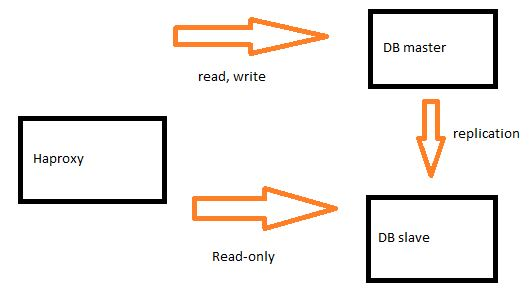
\includegraphics{../notes/img/networkdiagram_db_replication.JPG}
\caption{netwerk diagram}
\end{figure}

Er is nog uitbreiding mogelijk: Hoe van replica een master maken?

\hypertarget{donderdag-24032022}{%
\subsection{Donderdag 24/03/2022}\label{donderdag-24032022}}

Fysiek in Peutie

werkuren: \emph{8:00 - 16:00}

Introductie van \emph{mssql}\\
Onderzoeksopdracht besproken. ik zal hierover nog een document
ontvangen.\\
Tom heeft mij een rondleiding gegeven in de serverroom van in Peutie.

In de namiddag was er een drink binnen defensie waar de kolonel een
toespraak heeft gehouden. Het was tof om deze bij te wonen.

\end{document}

    
\end{document}